\chapter{Éléments de méthodologie}
\label{chap:method}

\lettrine[lines=3]{L}{e travail} présenté dans cette thèse repose sur de travaux
expérimentaux et théoriques. En particulier, la partie expérimentale est centrée sur l'étude de
populations de Collemboles de l'espèce \textit{Folsomia candida} élevées en
microcosmes au laboratoire. Dans ce chapitre, nous présenterons notre espèce
modèle du point de vu de sa biologie, de son intérêt pour les études menées, et
des conditions d'élevages. Puis nous détaillerons quelques développements
méthodologique qui ont permis l'accomplissement de nos travaux. 

\section{Le collembole, un modèle d'étude en écologie des populations}
\sectionmark{Le collembole modèle d'étude}

\subsection{Quelques généralités}

les Collemboles sont de petits arthropodes hexapodes entognathes aptères
mesurant généralement 1 à 5 mm. C'est un groupe très anciens qui compte
notamment l'un des plus vieux fossiles d'héxapode connu (\textit{Rhyniella
praecursor} 410 millions d'années). Aujourd'hui, plus de 8000 espèces ont été
décrites \autocites{bellinger2014a}, réparties dans l'ensemble des écosystèmes
terrestres connus, en faisant une des lignées d'arthropodes les plus communes au
monde.
Bien que proches des Insectes, les Collemboles forment une classe à part, à côté des
Diploures et des Protoures \autocites{grimaldi2010a}. Ils sont
classés en quatre ordres: les Poduromorphes, les Entomobryomorphes, les
Symphypléones et les Néanuridés.

Les Collemboles se distinguent de leurs groupes frères par plusieurs
caractéristiques qui leur sont propres. En particulier, on note la présence
d'un organe de saut, la furca, à l'extrémité de l'abdomen. La furca est
habituellement repliée sous l'abdomen, retenue par le rétinacle. L'ouverture du
rétinacle relâche la furca, ce qui propulse le collembole sur plusieurs
centimètres. Certaines espèces de collemboles ont perdu secondairement cet
organe. On note également la présence d'un tube ventral, essentiel dans la
régulation de l'équilibre osmotique des individus.

Répandus dans l'ensemble des écosystèmes terrestres à toutes les latitudes, les
collemboles vivent généralement dans le sol où ils
peuvent atteindre des densité jusqu'à plusieurs dizaines de milliers d'individus
par $m^2$. Il se nourrissent principalement de déchets organiques présents dans
la litière, ou d'hyphes de champignons, et participent ainsi au recyclage de la
matière organique.

Les collemboles sont amétaboles et sont caractérisés par un développement direct
et une reproduction itéropare. Les juvéniles sont semblables aux adultes et ne
diffèrent que par leur taille.
De parts leur mode de respiration cuticulaire, ils sont extrêmement sensibles à
l'humidité relative de leur environnement, et se regroupent généralement dans
les microcosmes les plus humides de leur habitat. 

\subsection{Le Collembole \textit{Folsomia candida}}

\subsubsection{Présentation}

\begin{figure}[!ht]
\begin{center}
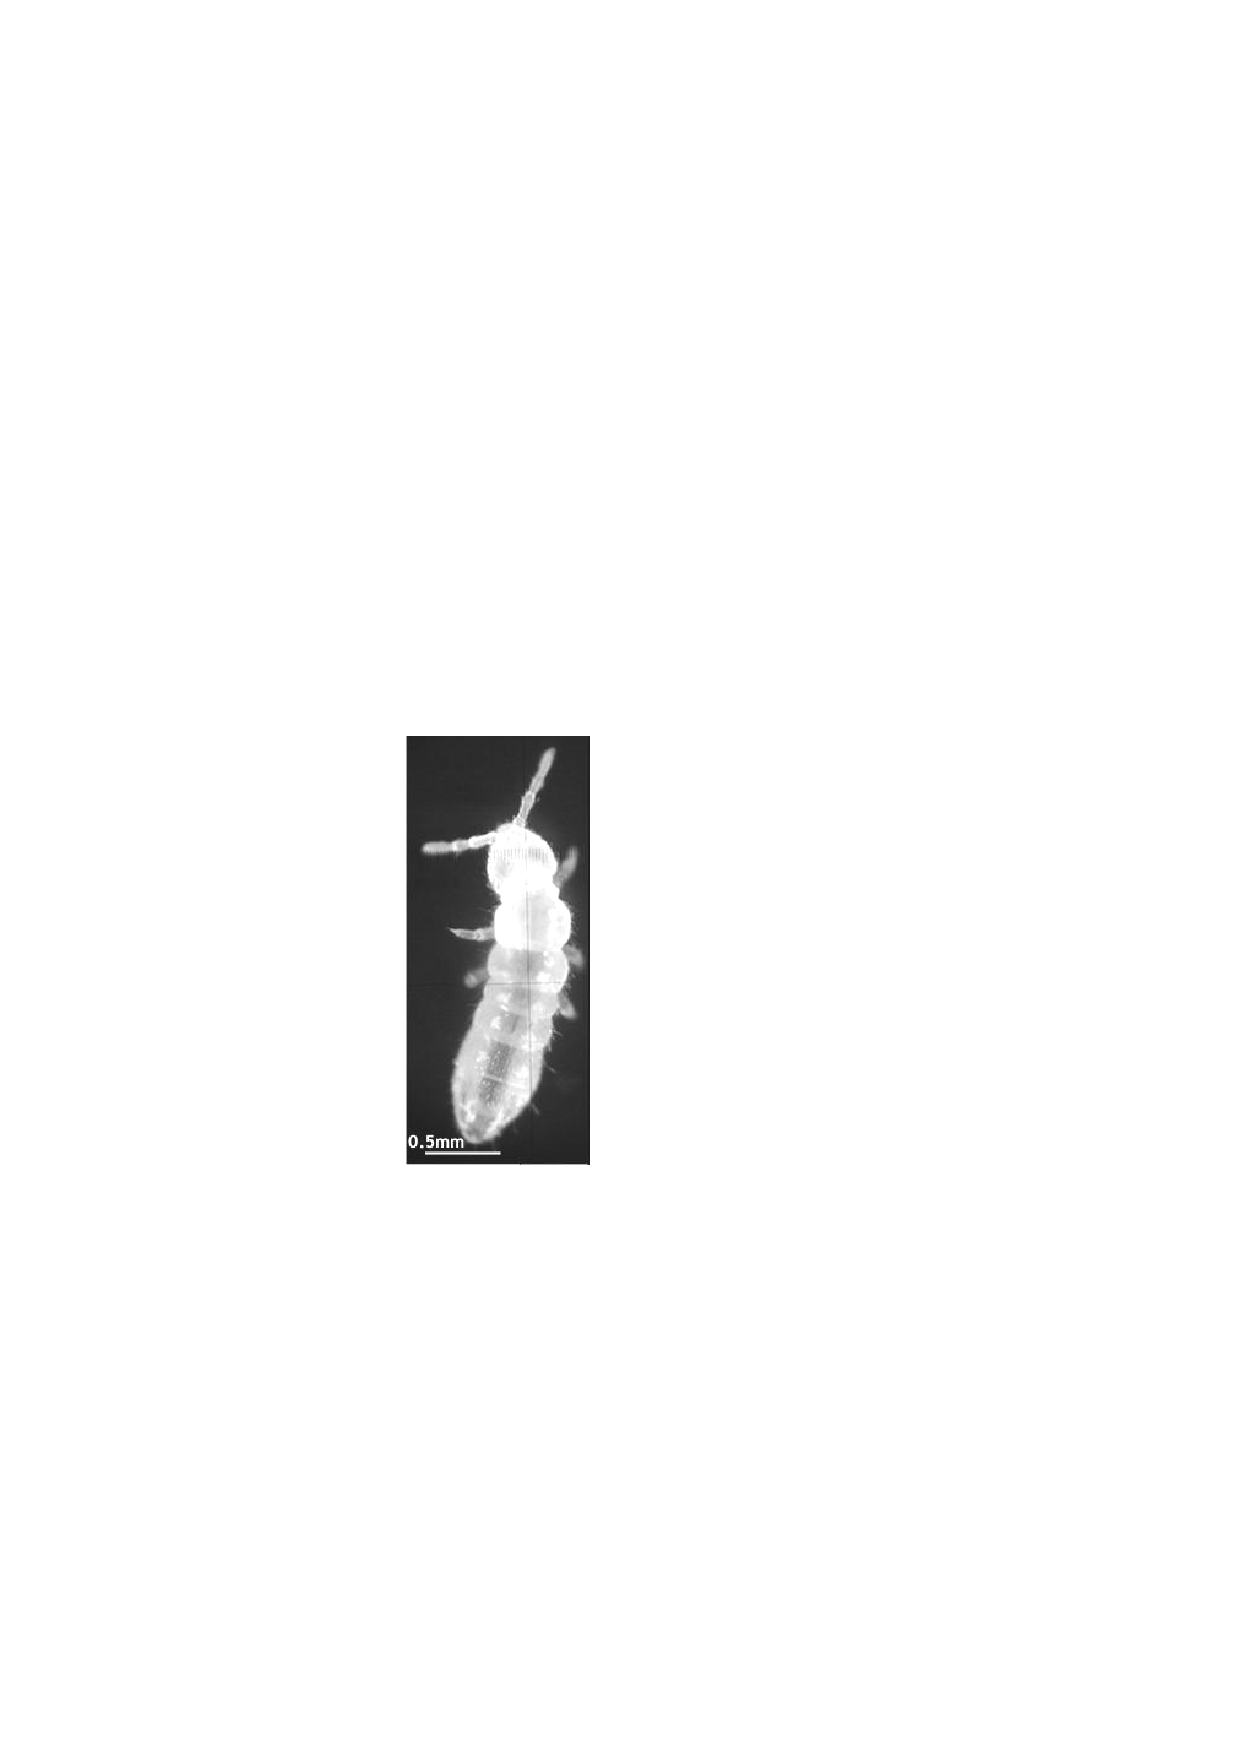
\includegraphics[width=3cm,angle=90]{1_CorpsDeThese/Methodo/folsomiacandida.pdf}
\caption[\lofimage{1_CorpsDeThese/Methodo/folsomiacandida.pdf} Collembole
\textit{Folsomia candida}]{Collembole
\textit{Folsomia candida}}
\label{fig:folsomia}
\end{center}
\end{figure}


\textit{Folsomia candida} (Figure \ref{fig:folsomia}) est un représentant très
commun des Collemboles, que l'on retrouve dans le monde entier. Il s'agit d'un
Collembole \textit{Arthropléone} de la superfamille des \textit{Entomobryoidae}
et de la famille des \textit{Isotomidae}. Cette famille comprend plus de 1000
espèces.
Une des caractéristiques principales de la famille des \textit{Isotomidae} est
que les segments abdominaux sont de même taille, contrairement aux autres
familles où le 4ème segment est généralement plus grand.

\textit{Folsomia candida} vit principalement dans les couches profondes du sol
(euedaphique) et quelques fois dans des caves ou des grottes. Il est très
répandu mais difficile à observé car extrêmement sensible à la dessiccation. On
le retrouve couramment dans des bois morts en phase avancée de décomposition
dans un sol humide. C'est une espèce petite ($\approx 1 - 2 mm$) aveugle et
blanche qu'il est aisé de maintenir en laboratoire dans des boites de petites
dimension. 

\subsubsection{Mode de reproduction}

La grande majorité des populations de collembole \textit{Folsomia candida} est
composé exclusivement de femelles dont la reproduction est parthénogénétique.
Cependant, certaines populations possèdent des mâles rares avec une reproduction
sexuelle facultative, et d'autre sont encore strictement sexuées. Chez
\textit{Folsomia candida} la parthénogénèse est possible grâce à l'infection par
la bactérie \textit{Wolbachia} qui permet vraisemblablement la duplication de
l'ADN dans l'oeuf sans division cellulaire, et ainsi à l'oeuf de passer d'un
état haploïde à un état diploïde sans fécondation. 

Ce mode de reproduction conduit à des lignées génétiques distinctes dont les
trajectoires évolutives sont diversifiées, conduisant aujourd'hui à des
populations aux stratégies d'histoires de vie parfois contrastés
\autocites{tully2004a,tully2008a}. Dans ces travaux de thèse,
\textcites{tully2004a} a réalisé une classification de 11 lignées clonales
issues de zones géographiques différentes. Cette classification a permis de
distinguer deux clades dont les stratégies d'histoires de vie sont très variées.
Au cours de cette thèse, nous nous sommes intéressés à deux lignées génétiques à
reproduction clonale, issues chacune d'un clade différent, ``HA'' et ``TO''. Ces
deux lignées nous permettent de comparer les réponses à la compétition par interférence et à la
température de populations aux stratégies biodémographiques contrastées.

\subsubsection{Croissance et reproduction continues}

Comparée à d'autres espèces couramment utilisées en écologie, \textit{Folsomia
candida} présente plusieurs avantages en tant qu'espèce modèle, en particulier
lorsque l'on s'intéresse aux traits d'histoire de vie comme la taille corporelle
qui détermine la dynamique de la structure de la population.
Les collemboles de cette espèce se développent toute leur vie dans le même
environnement en consommant la même ressource (amétabole). Il ne possèdent ni
stade larvaire, ni stade immobile, et seule la taille des individus différencie
les juvéniles des adultes. Cela permet de maintenir l'ensemble de la population
dans un environnement contrôlé sans avoir à séparer les individus par leur
stade. De plus, il n'a pas été rapporté de cannibalisme au sein des populations,
et le régime alimentaire constant au cours de la vie permet de maintenir des
populations en environnement contrôlé pendant plusieurs années. Les individus
poursuivent leur croissance toute au long de leur vie par mue successive, et une
fois la maturité atteinte, se reproduisent pendant une très large majorité de
leur vie (la reproduction comme les autres traits étant soumise à sénescence).

\begin{figure}[!ht]
\begin{center}
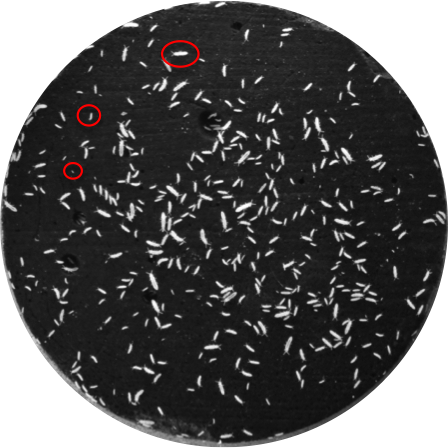
\includegraphics{1_CorpsDeThese/Methodo/StrucTaille}
\caption[\lofimage{1_CorpsDeThese/Methodo/StrucTaille} structuration en taille
d'une population de collemboles.]{Illustration de la structuration en taille
d'une population de collemboles. Les cercles rouges montrent trois tailles
différentes de collembole.}
\label{fig:strucpop}
\end{center}
\end{figure}

Ce mode de développement continu tout au long de la vie et la facilité
d'élevage en laboratoire (décrite ci-après) font du collembole une espèce
particulièrement adaptée à l'étude de la dynamique des populations structurées
(Figure \ref{fig:strucpop}).
Des suivis fins de plusieurs populations nous permettrons l'étude des
problématiques expérimentales et la paramétrisation du modèle dans l'étude
théorique. 

\subsection{Modalités d'élevage au laboratoire}

Les méthodes d'élevage au cours de chacune de nos expériences sont issues du
protocole développé par \textcites{tully2004a} pendant sa thèse.

\subsubsection{Boites d'élevage}

Les collemboles sont maintenus dans des boites cylindriques en
plastique transparent de $5.1 cm$ de diamètre fermées avec un couvercle de
couleur permettant de codifier la lignée clonale présente dans la boite, et dont
le fond a été troué. Les boites sont remplies d'un substrat de pâtre de Paris de
$3cm$ peint en noir à l'encre de chine Pebeo\textcopyright. Ce plâtre est
réalisé suivant la recette de la Table \ref{tab:recettes}a. Le plâtre imbibé
d'eau permet de maintenir une humidité relative proche de $100\%$ à la surface.

\begin{table}[!h]
\begin{center}
\begin{tabular}{rl|rl}
\multicolumn{2}{c}{(a)Substrat de plâtre}&\multicolumn{2}{c}{(b) Pastilles de levure}\\
\hline 
$37mL$ & d'eau & $5mL$ & d'eau\\ 
$1mL$ & d'encre de Chine & $0.08g$ & d'agar agar \\ 
$50g$ & de plâtre de Paris & $0.8g$ & de levure de bière\\
& & $150\mu L$ & de colorant\\ 
\end{tabular} 
\caption[Recettes]{\label{tab:recettes}Recettes}
\end{center}
\end{table}

Préalablement au démarrage d'une population, les boîtes d'élevage sont
humidifiées en les trempant dans de l'eau. L'humidification du plâtre peut être
contrôlée en vérifiant sa teinte qui devient plus foncée lorsqu'il absorbe
l'eau. L'épaisseur du substrat de plâtre permet d'absorber suffisamment d'eau
pour qu'une population dans une boîte fermée puisse être conservée plusieurs
mois sans manipulation.

\subsubsection{Nourriture}

Les populations sont nourries une fois par semaine. Afin de contrôler
précisément la quantité de ressource apportée, les populations sont nourries
avec une de pastille de $15\mu L$ d'un mélange de levure de bière déshydratée et
d'agar-agar (cf. Table \ref{tab:recettes}b).

\subsubsection{Contrôle de la température et manipulation des boites d'élevage}

Les boites d'élevage sont maintenue à température constante ($\pm 0.5\degres C$)
dans des étuves dans le noir. Toutes les populations expérimentales étudiées
dans cette thèse ont été élevées dans ces conditions, et n'ont été manipulées
que lors des opérations de comptage ou de nourissage. Au cours de l'expérience
présentée dans le Chapitre \ref{chap:sm}, les boîtes ont été changées au moment
de la perturbation de la structure. Toutefois, si une boîte s'est trop
dégradée au cours du temps (développement de moisissures et de
champignons notamment), elle est changée pour une nouvelle boite
propre. Bien qu'un soin particulier ait été apporté à cette opération pour
impacter au minimum les populations concernées, cette manipulation constitue une
 perturbations exceptionnelles des conditions d'élevage pouvant avoir un impact
 sur la dynamique de la population (cf. Chapitre \ref{chap:sp}).

\section{Phenotypage haut débit des populations}
\label{sec:bpsensor}

L'étude de la dynamique de la structure des populations de collemboles nécessite
une mesure non invasive mais précise de la structure au cours du temps. De plus,
cette mesure doit pouvoir être répétée un grand nombre de fois sans difficulté,
soit pour des populations différentes afin de multiplier les réplicats ou les
conditions testées, soit dans le temps pour accumuler suffisamment de données
pour avoir des séries temporelles exploitables. Ces besoins spécifiques de
précision et d'efficacité nous ont conduit à développer une méthode
semi-automatisée de dénombrement des populations et de mesures des individus.
Cette mesures se base sur l'analyse automatique de photographies standardisées
des populations \autocites[Figure
\ref{fig:photocount}, ][]{mallard2012a,mallard2013a}.

\begin{figure}[!ht]
\begin{center}
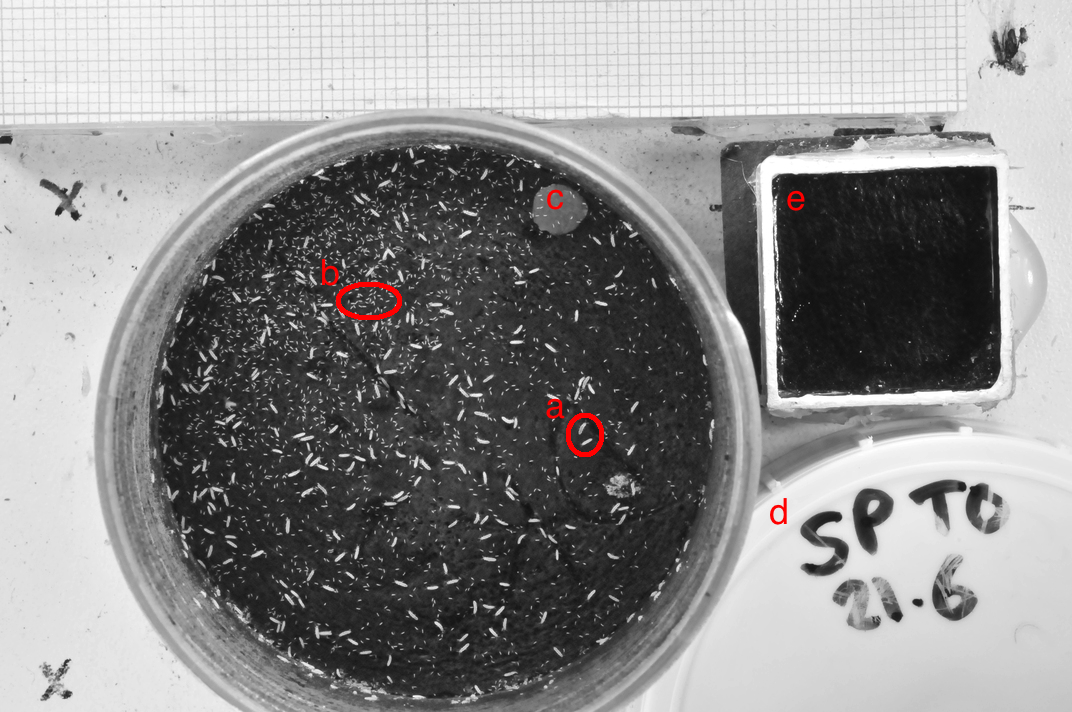
\includegraphics[width=0.85\textwidth]{1_CorpsDeThese/Methodo/PhotoCount}
\caption[\lofimage{1_CorpsDeThese/Methodo/PhotoCount} Photo d’une boite pour le
comptage et la mesure des individus]{Photographie d'une boite pour le comptage
et la mesure des individus. Cette population contient des individus de toutes
tailles, des adultes (a) aux jeunes fraîchement éclos (b). La pastille de
nourriture est également visible (c). La boite est repérée par un code unique
(d) contenant le code d'expérience (SP), la lignée (TO), la température
d'élevage ($21\degres C$) et le numéro de boite (6). Le carré noir (e) sert
d'échelle pour la mesure des individus}
\label{fig:photocount}
\end{center}
\end{figure}

Les progrès incessant en matière de photographie numérique et de capacité de
stockage de données ont radicalement changé la façon dont les chercheurs
utilisent l'image pour acquérir et stocker des données \autocites{walter2005a}.
Parallèlement, de nombreux outils se sont développés pour traiter ces données
\autocites{eliceiri2012a,schneider2012a}. En écologie théorique, ces progrès ont
permis l'acquisition de larges jeux de données de comportements individuels, de
fécondités ou de trajectoires de croissance avec une très bonne résolution
temporelle. Mais le traitement de ces jeux de données reste long et peut
rapidement devenir infaisable. 

Plusieurs solutions ont déjà été proposées pour traiter automatiquement des jeux
de photographies, ou dénombrer des populations de petits organismes
\autocites{hooper2006a,krogh1998a,auclerc2010a,lukas2009a,marcal2006a}. Mais ces
méthodes ne permettent pas de prendre en compte l'hétérogénéité du substrat de
plâtre qui emplit nos boîtes d'élevage, ni ne fait la différence entre des
individus vivant et  morts ou des particules parasites sur le fond de la
boîte, très communes dans nos populations (morceaux de pastilles de
nourritures, mues, oeufs,\ldots). Nous avons donc développé une méthode
d'analyse d'image permettant de prendre en compte ces considérations, et
d'améliorer la fiabilité des mesures de taille individuelle et de densité des
populations sur un substrat hétérogène. Le principe de notre méthode repose sur
un plugin du logiciel de traitement d'image ImageJ appelé multi-tracker
\autocites{schneider2012a,kuhn2001a}.

\subsection{Méthode}

\begin{figure}[!ht]
\begin{center}
\includegraphics[width=0.55\textwidth]{1_CorpsDeThese/Methodo/1_collemboles_etapes}
\caption[\lofimage{1_CorpsDeThese/Methodo/1_collemboles_etapes} Les étapes
de l'analyse d'image]{Les étapes successives de l'analyse d'image (exemple
d'une population de collemboles).
(a) Deux photos extraites de la série d'images. (b) Le fond de l'image
reconstruit. Chaque pixel est sélectionné comme étant le plus sombre de la
pile d'image à cette position. (c) On soustrait le fond (b) à l'image de départ
(a) pour retirer le fond immobile et révéler les éléments mobiles. Le point blanc
(flèche en b) a été éliminé. (d) Après sélection de la limite d'intensité, on
peut compter et mesurer facilement chacune des particules.}
\label{fig:photoetapes}
\end{center}
\end{figure}



Le principe de base de la méthode développée consiste à comparer plusieurs
photographies du même microcosme prises à quelques secondes d'intervalle, en
gardant l'ensemble du dispositif immobile. Cela permet d'obtenir une série
d'images de la même population où seuls les éléments mobiles au cours de la
prise de vue diffèrent entre les images. Cette série d'image est appelée une
``pile''.
Généralement, trois à cinq photos sont suffisantes pour que tous les individus
vivants aient bougé entre au moins entre la première et la dernière photo de la
série (Figure \ref{fig:photoetapes}a).

Au cours de nos expériences, l'ensemble des photos utilisées pour les suivis
de populations ont été prises avec un appareil photo réflex piloté par
ordinateur (Nikon D300 et CameraControlPro\textcopyright). Il est également important de disposer d'un
éclairage stable afin que les conditions d'éclairage des prises de vue soient
constantes entre toutes les photos. Nous avons utilisé des ampoules à LED afin
de limiter les risques de fluctuation d'éclairage au cours du temps. 

Une fois la pile d'image obtenue, pour chacune des positions possibles, on
sélectionne dans la pile d'image le pixel le plus sombre. Les collemboles
étant clairs sur un fond sombre, on reconstruit ainsi une image composite qui
contient uniquement les éléments les plus sombres et ceux immobiles au cours de
la prise de vue (Figure \ref{fig:photoetapes}b).
Ainsi, il suffit que tous les pixels de l'image soit au moins une fois sans collembole
dans la série de photos pour que l'image composite représente fidèlement le
``fond'' de la boite. Si un élément clair (une mue par exemple) est présent sur
le substrat, s'il est strictement immobile, il sera également sélectionné comme
fond de l'image (flèche sur la Figure \ref{fig:photoetapes}b). 
On peut alors soustraire le fond immobile de chacune des photos de départ pour
obtenir des images ne contenant que les éléments mobiles (Figure
\ref{fig:photoetapes}c). 

La dernière étape consiste alors à convertir les images en image 8-bits (256
niveaux de gris), et à sélectionner le niveau de gris qui permettra de faire la
différence entre les collemboles et le reste de l'image (limite d'intensité,
Figure \ref{fig:photoetapes}d). Cela crée une image 2-bits (noir ou blanc) sur
la quelle le logiciel ImageJ peut détecter les contours et mesurer les
particules (pour nous les collemboles). A cette étape, le logiciel nous permet
d'obtenir la taille et la surface de chacune des particules présentes sur
chacune des photos analysées.

Cette série d'opération a été automatisée dans un plugin afin de bénéficier d'un
rendement accru dans le traitement des images. Grâce à ce plugin, un grand
nombre de populations peuvent être mesurées en peu de temps et sans
interventions. Pour chacune des populations, le plugin fournit en sortie un
tableau contenant une ligne par particule mesurée, et en colonne des
informations telles que le nom de la photo (afin d'accéder à la date de prise
de vue et aux codes de l'expérience), la longueur des particules, leur
surface, \ldots

\subsection{Fiabilité de la méthode}

Nous avons testé notre méthode sur différents critères \begin{enumerate*}[label=(\roman*), before=\unskip{ : }, itemjoin={{ ; }},
itemjoin*={{ ; et }}] 
\item le nombre d'image nécessaires au calcul du fond
\item la répétabilité de la mesure de la structure de la population
\item la fiabilité du dénombrement de la population
\end{enumerate*}

\begin{figure}[!ht]
\begin{center}
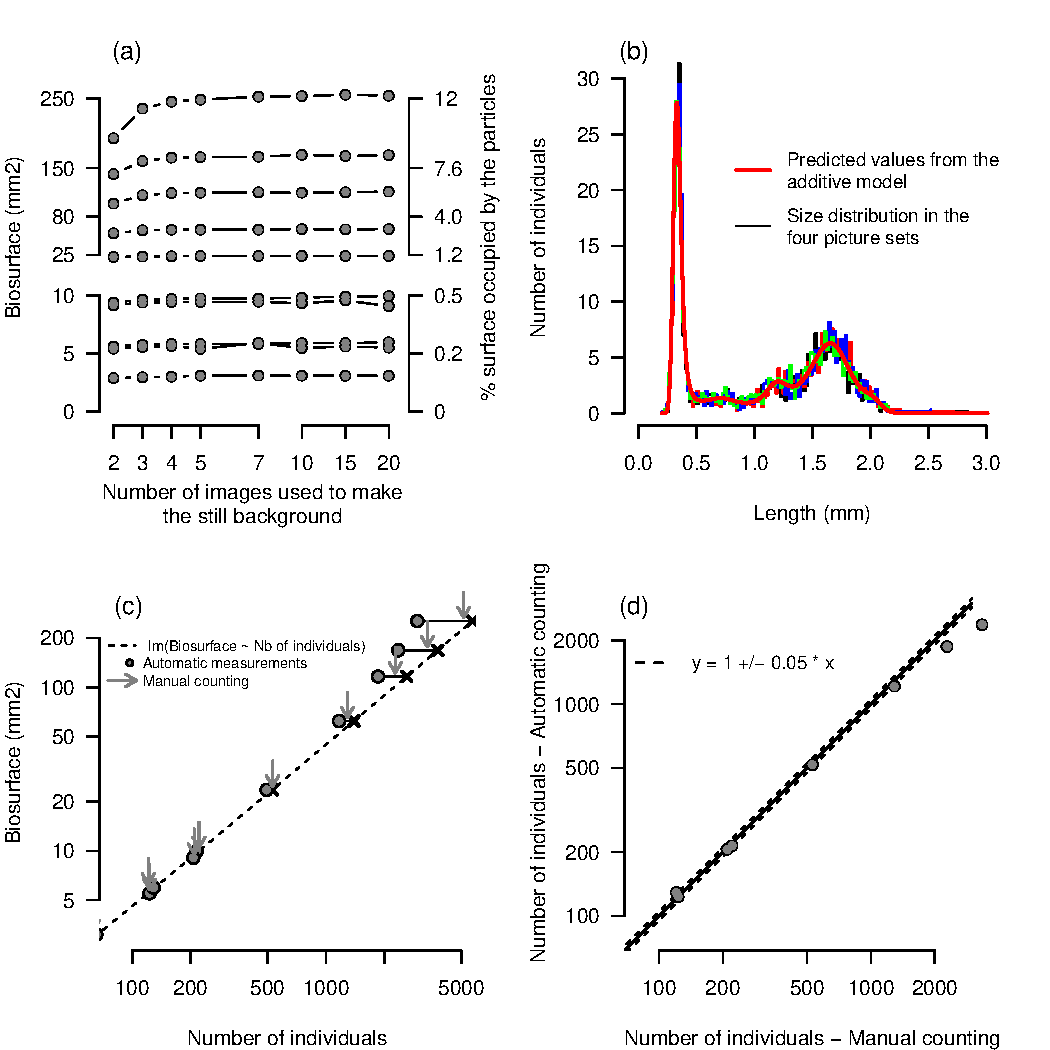
\includegraphics[width=0.80\textwidth]{1_CorpsDeThese/Methodo/6_Plugin_multiP}
\caption[\lofimage{1_CorpsDeThese/Methodo/6_Plugin_multiP} Analyse de la
fiabilité]{Analyse de la fiabilité de la méthode de mesure. (a) Biosurface
totale de collemboles mesurée ($mm^2$) en fonction du nombre de photos utilisés
pour constituer le fond. (b) Distribution en taille d'une même population de
collemboles mesurée quatre fois indépendemment par deux utilisateurs
différents, la ligne rouge représente un modèle général additif qui ne montre
aucune différence significative entre les photos ou les séries de mesures. (c)
Biosurface en fonction du nombre d'individus (cercles) comptés automatiquement,
les flèches montrent le nombre d'individus comptés à la main, la ligne
pointillée représente une régression linéaire sur les premiers points de mesure.
(d) Comparaison du nombre d'individus comptés automatiquement et à la main. }
\label{fig:photofiabi}
\end{center}
\end{figure}

\subsubsection{Nombre d'image pour le calcul du fond}

Dix populations contenant des densités croissantes d'individus de $0.25$ à
$0.5mm$ ont été prises en photos dans les conditions décrites précédemment avec
des séries de 20 photos. La biosurface d'individus (surface occupée sur la photo
par les individus) a été mesurée pour chacune des dix populations en utilisant
un nombre croissant d'image pour le calcul du fond. Si la densité d'individus est
élevée dans la populations, un plus grand nombre de photos sont nécessaires pour
obtenir une image fidèle du fond de la boite, dépourvue d'individus mobiles qui
auraient du être éliminés. Bien qu'à faible densité le nombre de photos
utilisées pour le fond de la boite ait peu d'effet sur la mesure de densité, à forte
densité, les mesures répétées dans les populations montrent que la biosurface
mesurée augmente avec le nombre d'image utilisées pour fabriquer le fond
(Figure \ref{fig:photofiabi}a). Il faut un minimum de quatre à cinq images à
très fortes densités pour obtenir une mesure fiable. En revanche il n'est pas
nécessaire d'utiliser plus que six images pour établir le fond, la mesure
de densité n'en étant pas améliorée. 

\subsubsection{Répétabilité de la mesure de la structure en taille}

Quatre jeux de cinq photos ont été analysés. Deux utilisateurs différents ont
pris chacun deux jeux de photos à quelques minutes d'intervalle pour assurer
l'indépendance des mesures. Les distributions en taille mesurées pour chacun des
quatre jeux de photos sont alors superposées et comparées en utilisant un modèle
additif autorégressif (Figure \ref{fig:photofiabi}b). Les quatre distributions
obtenues se recouvrent largement et aucune différence significative n'a pu être
mise en évidence. Notre méthode permet donc une mesure fiable et répétable de la
structure en taille des populations de collemboles.

\subsubsection{Fiabilité du dénombrement}

Le nombre de particules et leur surface ont été comptés avec la procédure
automatique sur dix populations de densités croissantes. Ces mesures
automatiques sur des jeux de vingt photos ont ensuite été comparées à des comptages manuels
du nombre d'individus. 

En dessous de 1000 individus, notre méthode de comptage d'individus présente une
remarquable fiabilité (Figure \ref{fig:photofiabi}d). Au delà de cette densité,
le nombre d'individus comptabilisés par la méthode automatique est de plus en
plus sous-estimé par rapport au comptage manuel. En effet, lorsque la densité
augmente, de plus en plus d'individus se touchent sur les photos et sont alors
détectés comme une seule grosse particule. La biosurface devient alors un
meilleur proxy pour le nombre d'individu à supposer que tous les individus aient
une taille similaire, ce qui est le cas dans cet exemple. On peut alors projeter
la relation entre biosurface et nombre d'individus obtenue à faible densité pour
les fortes densités et ainsi connaitre le nombre d'individus en mesurant la
biosurface (Figure \ref{fig:photofiabi}c).

\subsection{En conclusion}

En conclusion, cette méthode présente une grande fiabilité et permet d'accéder à
moindre coût à plusieurs mesures au sein des populations de collemboles pour une
perturbation minimale. Pour cette thèse, cette méthode permet d'accéder au
nombre d'individus ainsi qu'à la longueur corporelle et la biosurface de chacun
des individus, donnant ainsi une mesure de la structure des populations. 

De plus l'implémentation automatisée de la méthode permet de mesurer un grand
nombre de population dans un temps réduit. Une centaine de populations sont
ainsi dénombrées en environ trois heures sur un ordinateur dual-core cadencé à
$2.5GHz$ (à raison de $20$ à $30s$ par jeu de 5 photos).

D'autre part, cette méthode peut également être appliqué à d'autres organismes
ou systèmes expérimentaux. Plusieurs exemples d'utilisation sont décrits en
détail en annexe (voir Annexe \ref{chap:bpsensor}).

\section{Méthode de représentation graphique}\label{sec:stdiag}

Notre méthode automatisée d'analyse d'image pour le dénombrement et la mesure de
la structure en taille des populations de collemboles nous permet d'accumuler
rapidement un grand nombre de données. Précisément, à chaque date de mesure nous
disposons pour chacune des populations étudiées du nombre d'individus, et pour
chacun des individus de sa taille corporelle et de sa biosurface. Au cours
de nos expérimentations, nous avons été amenés à suivre plusieurs dizaines de
populations durant plusieurs dizaines de semaines. Face à ces jeux de données de
grande taille, il a été nécessaire de développer des techniques de
représentation et d'analyse spécifique afin d'être capable d'extraire l'ensemble
des informations présentes. Nous avons donc mis en place une méthode graphique
simple permettant la représentation de la dynamique temporelle de la structure
d'une population. 

\begin{figure}[!ht]
\begin{center}
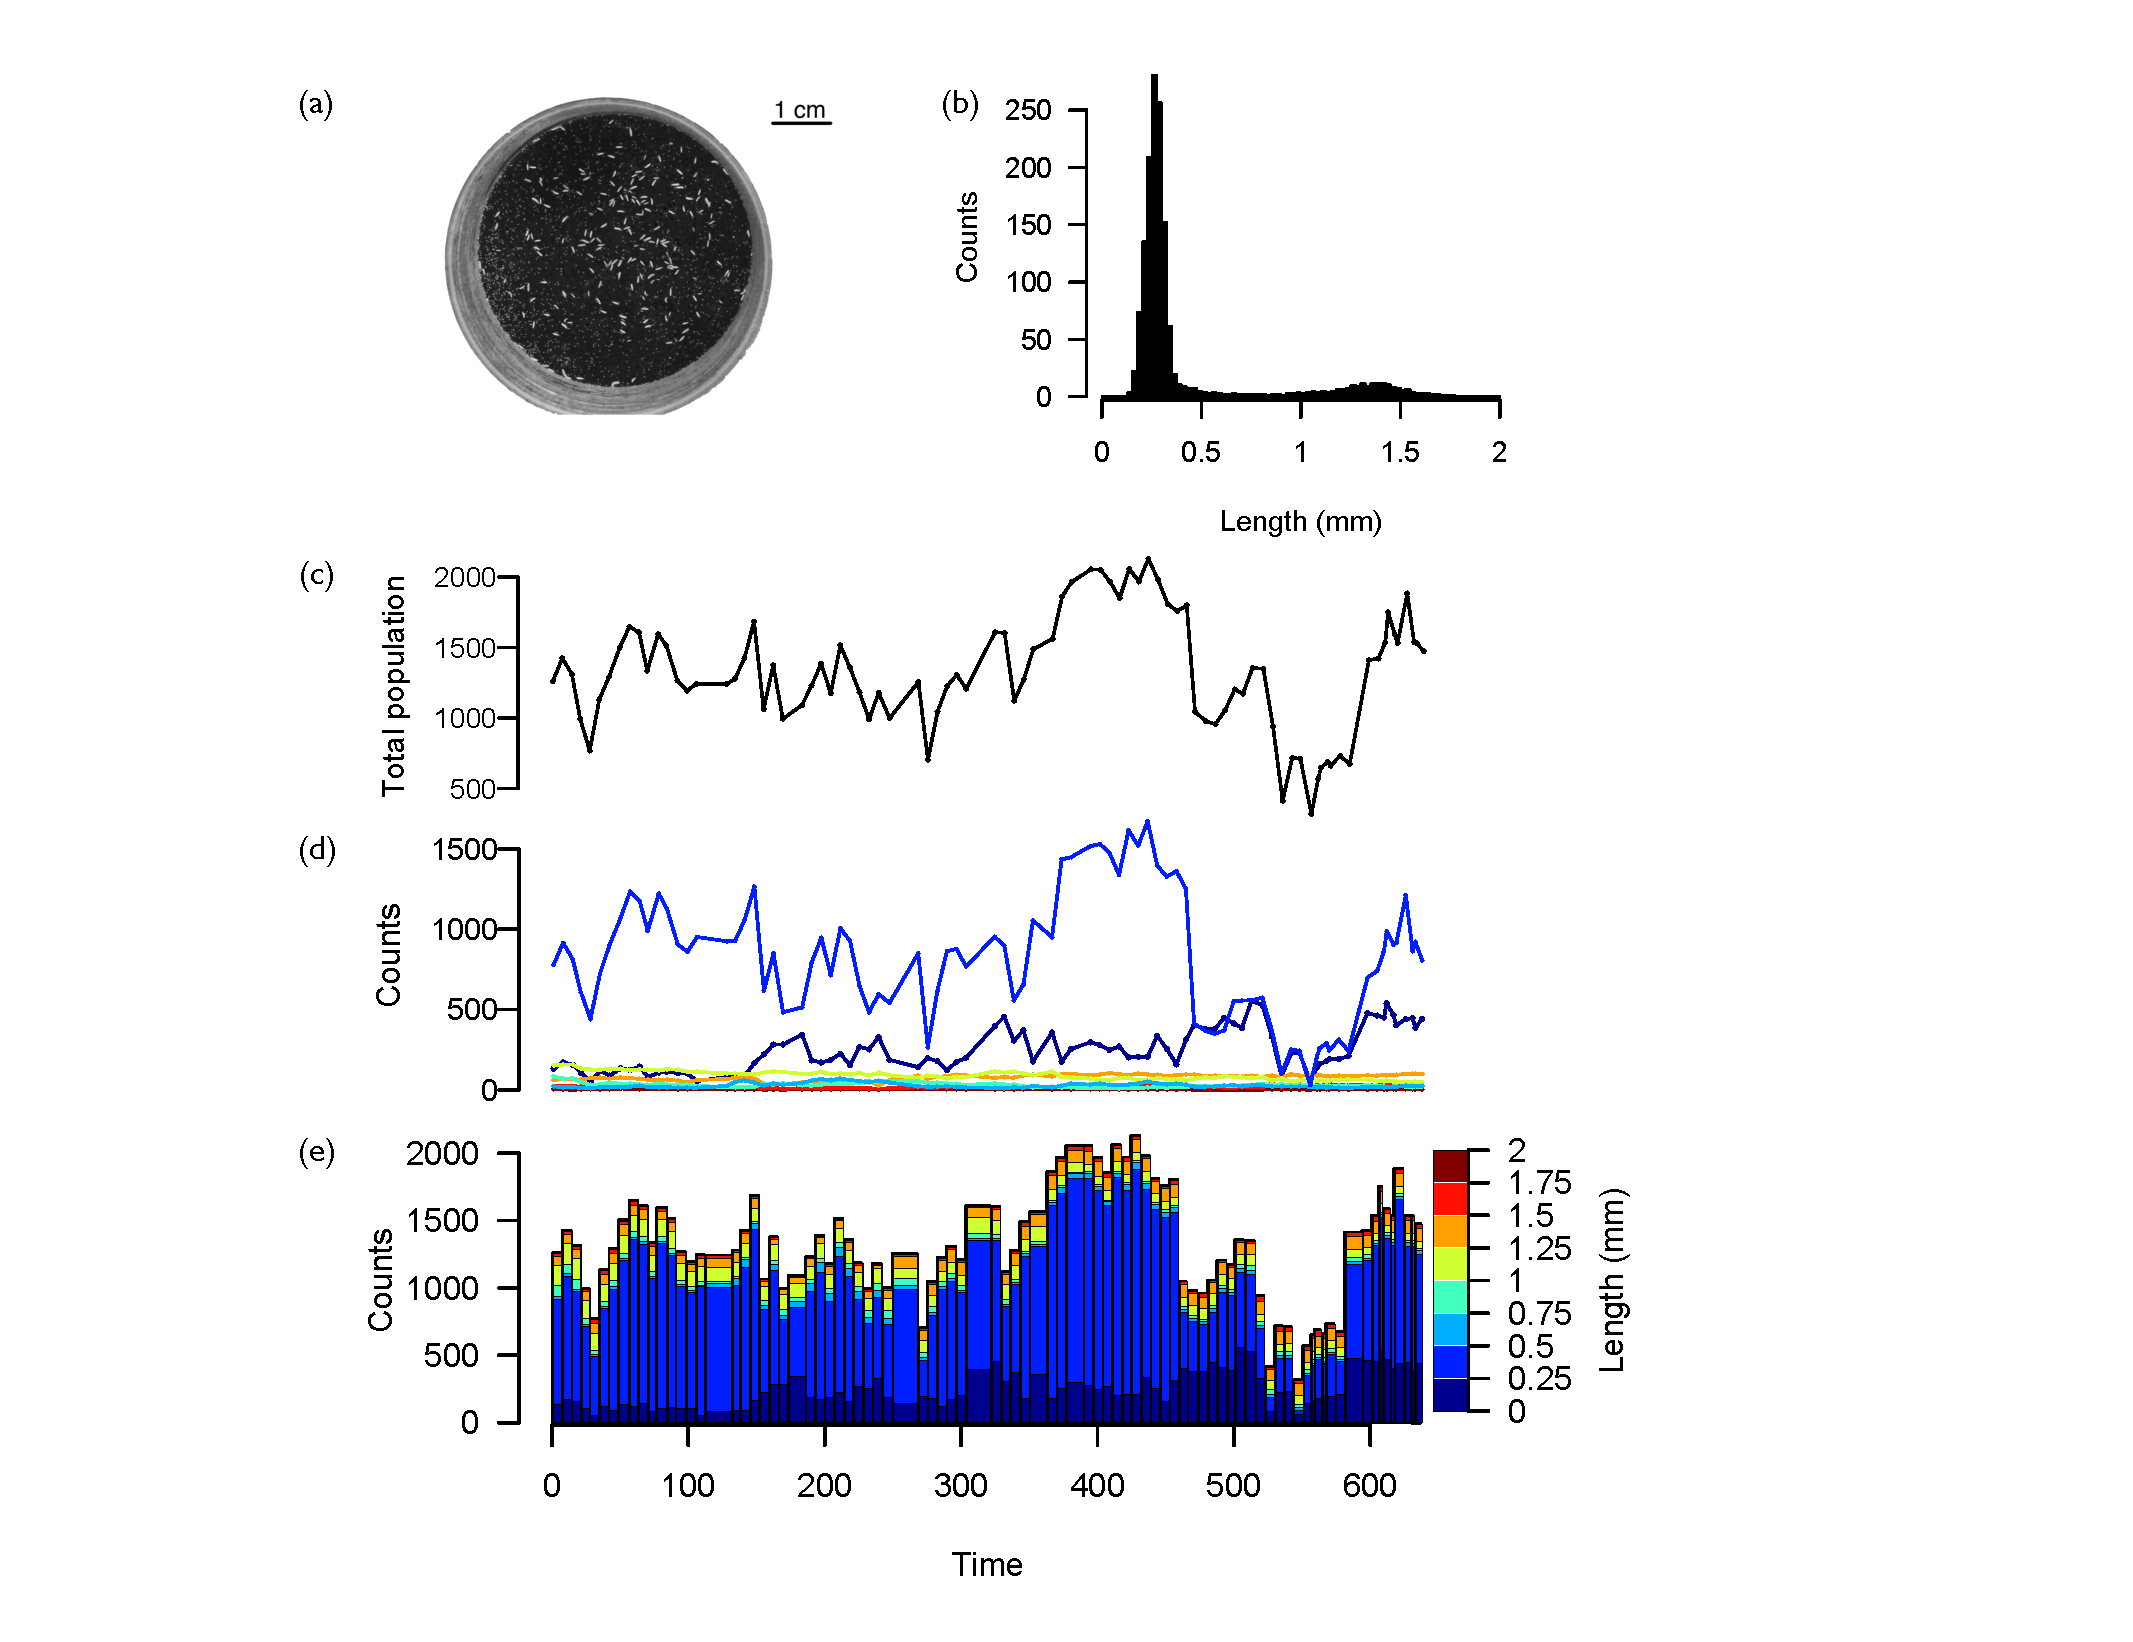
\includegraphics[width=0.85\textwidth]{1_CorpsDeThese/Methodo/STdiag1}
\caption[\lofimage{1_CorpsDeThese/Methodo/STdiag1} Représentation de la
structure d'une population]{Exemple de représentations classiques de la
structure d'une population de collembole \textit{Folsomia candida}. (a)
Photographie de la population. (b) A une seule date, la structure est
classiquement représentée par un histogramme de la taille corporelle. (c)
Dynamique de la population totale. (d) Pour représenter à la fois la structure
et sa dynamique, la population a été divisée en classes de taille et leur
dynamiques ont été tracées sur le même graphique indépendemment, ou (e)
empilées. Ces représentations montrent la dynamique globales et au sein des
classes définies a priori, mais ne montrent pas les dynamiques transversales.}
\label{fig:STd1}
\end{center}
\end{figure}

Plusieurs approches sont couramment utilisées pour décrire la dynamique de
populations structurées (Figure \ref{fig:STd1}c-e) en représentant par exemple
la dynamique de la population dans son ensemble, sans prendre en compte la
structure \autocites[Figure \ref{fig:STd1}c, ][]{schrautzer2011a}. La structure
peut être prise en compte grossièrement en séparant les individus en classes de
taille (ou de stade) arbitraires et en représentant ces dynamiques sur des
graphiques séparés \autocites{plaistow2009a} ou sur le même graphique en superposant les
courbes pour faciliter la comparaison (Figure \ref{fig:STd1}d) ou à l'aide d'une
représentation empilée pour faire ressortir la dynamique globale
\autocites[Figure \ref{fig:STd1}e,][]{madsen2000a}. Mais cette méthode ne permet
de comparer et d'étudier qu'un petit nombre de classes pour conserver de la
lisibilité. 

Si l'élément structurant de la population est continu, comme c'est le cas
pour la taille corporelle chez les collemboles, il est nécessaire d'opter pour
une représentation à trois dimensions (le temps, l'élément structurant et une
mesure de la densité d'individus) pour représenter finement la dynamique de la
structure de la population. Parmi ces représentations, on retrouve notamment les
diagrammes dits ``event history diagrams'' qui représentent les traits
d'histoire de vie individuels au niveau de l'ensemble d'une cohorte
\autocites{carey1998a,carey2008a}, ou les diagrammes colorés (``shaded contour
maps'') tels que ceux utilisés pour représenter la dynamique temporelle de taux
vitaux dépendant de l'âge \autocites[mortalité ou natalité chez les humains par
exemple,][]{vaupel1997a,vaupel1998a}. Ces représentations sont
principalement utilisées chez les humains pour montrer des changements séculier
dans des taux démographiques dépendant de l'âge
\autocite{vaupel1987a,vaupel1997a,vaupel1998a,andreev2000a,erlangsen2003a}.

A notre connaissance, ce type de représentations colorées n'a pratiquement
jamais été utilisé en écologie pour représenter la dynamique temporelle de la
structure d'une population. Nous avons développé une suite d'outils pour le
logiciel de statistique R \autocites{team2012a} spécifiquement
orientés vers les données de populations structurées permettant la manipulation
des données, leur représentation graphique et quelques manipulations simples sur
ces graphiques. Ces outils sont disponibles dans une librairie R appelée
\texttt{STdiag}. Cette librairie est téléchargeable à l'adresse
\url{http://r-forge.r-project.org/projects/stdiag}.
Nous détaillerons dans cette section comment utiliser cette librairie pour
générer les graphiques et discuterons brièvement de leur intérêt pour l'écologie
des populations. 

\subsection{Méthode}

Dans la suite de cette thèse, les diagrammes produits avec cette méthode seront
appelés ``diagrammes structure-temps''. Cette nomenclature vient du fait que ces
diagrammes représentent le temps en abscisse et l'élément structurant en
ordonnées. Pour chaque date de mesure, on représente sur un histogramme codé par
une échelle colorée le nombre d'individus le long de l'élément structurant. La
taille des classes utilisées pour les histogrammes dépend de la qualité et de la
précision des données. Dans notre cas, les mesures de taille dans les
populations de collemboles sont discrétisées en classes de $0.1mm$ entre $0$
et $3mm$. Bien que l'on discrétise encore des données continues, cette méthode
permet d'avoir une bien meilleure résolution qu'avec les méthodes décrites
précédemment car on peut conserver une grand nombre de classes de tailles sans
difficultés (dans notre cas 30 classes). De plus, en utilisant la même
discrétisation pour toutes les dates de mesures et en juxtaposant les
histogrammes obtenus, on obtient alors une représentation visuelle de la
dynamique de la structure de la population. 

Le package \texttt{STdiag} peut être installé dans R avec la commande :
\begin{verbatim}
install.packages('STdiag',repos="http://r-forge.r-project.org")
\end{verbatim}

La librairie fourni un jeu de données en exemple, \texttt{sample} que nous
utiliserons pour illustrer l'utilisation et l'intérêt de la méthode. Les données
sont issues d'une population de collemboles élevée dans les conditions décrites
précédemment et dénombrée et mesurée avec notre méthode automatique. 

\subsubsection{Importation et formattage des données}

La fonction principale d'affichage est une interface de la fonction
\texttt{levelplot} du package \texttt{lattice} \autocites{sarkar2008a}. Le
format principale pour les données est donc le format \texttt{data frame} de R.
Les données sont alors organisées en 3 colonnes, X le temps, Y l'élément
structurant (pour nous la taille) et Z le nombre d'individus. Le tableau de
données a donc $T \times S$ lignes ou $T$ est le nombre de dates de mesures et
$S$ le nombre de classes de taille.

La fonction de tracé accepte également le format \texttt{matrix} tel qu'utilisé
par la fonction \texttt{image}. La librairie propose une fonction de
conversion du format matrice au format data frame (\texttt{Matrix2Dataframe}).

% La matrice contient alors les données de nombre
% d'individus et a pour dimensions $TxS$. On utilise alors un vecteur X de
% longueur $T$ et un vecteur Y de longueur $S$ pour préciser les coordonnées en
% temps et taille de chaque case de la matrice. La conversion du format matrice
% vers le format tableau de données est possible par la fonction
% \texttt{Matrix2DataFrame}.

Enfin, la fonction incluse \texttt{Indiv2DataFrame} permet de formatter des
données individuelles telles que celles fournies par notre méthode d'analyse
d'image en données utilisables par la fonction de tracer.
Cette fonction prend en entrée un tableau contenant une ligne par individu mesuré dans
une population et contient dans deux colonnes respectivement la date de la
mesure et la valeur de la mesure de l'élément structurant. On peut alors
contrôler le nombre de classe pour discrétiser les données avec l'argument
\texttt{classes} qui est soit un entier spécifiant le nombre de classes voulues.
Les classes sont alors découpées régulièrement pour contenir l'ensemble des
données fournies; soit un vecteur de longueur $nombre\,de\,classes + 1$
précisant les bords de chacune des classes de taille (comme pour l'argument
\texttt{breaks} de la fonction de base \texttt{hist}).

\subsubsection{Tracé du diagramme}

La façon la plus simple de tracer le diagramme est d'utiliser le format tableau
de données. En utilisant la syntaxe de formule, on peut préciser les éléments du
tableau de données à tracer:
\begin{verbatim}
STdiag(z ~ x * y, data=sample).
\end{verbatim}
Toutes les options classique de personnalisation du graphique sont disponibles,
notamment pour les légendes des axes, les titres, \textit{etc}.

\subsubsection{Amélioration du graphique}

Plusieurs options sont également disponibles pour améliorer la lisibilité du
diagramme. En particulier, il est possible de choisir différentes palettes de
couleur pour le nombre d'individus avec l'option \texttt{color}. Il est
également possible d'utiliser un axe colorimétrique suivant une échelle
logarithmique avec l'option \texttt{log=TRUE/FALSE}. 

Enfin, si les données ne sont pas régulières, il est possible des les interpoler
avec la fonction \texttt{Interpolation} fournie ou l'option
\texttt{interp=TRUE/FALSE} directement dans la fonction de tracé. Il faut
toutefois être prudent avec l'interpolation afin de ne pas risquer d'interpréter
des données fausses. Il est également possible de lisser la représentation en
traçant la densité en deux dimension calculée en utilisant une fonction dérivée
de la fonction \texttt{kde2d} de la librairie \texttt{MASS}. 

Les différentes possibilités d'amélioration graphiques sont illustrées par la
Figure \ref{fig:STd2}. Dans la suite de cette thèse, les diagrammes
structure-temps seront généralement réalisés en utilisant la palette de couleur
\texttt{tim.colors} (librairie \texttt{fields}) avec une échelle de couleur
logarithmique et sans interpolation ou lissage. 

\begin{figure}[!ht]
\begin{center}
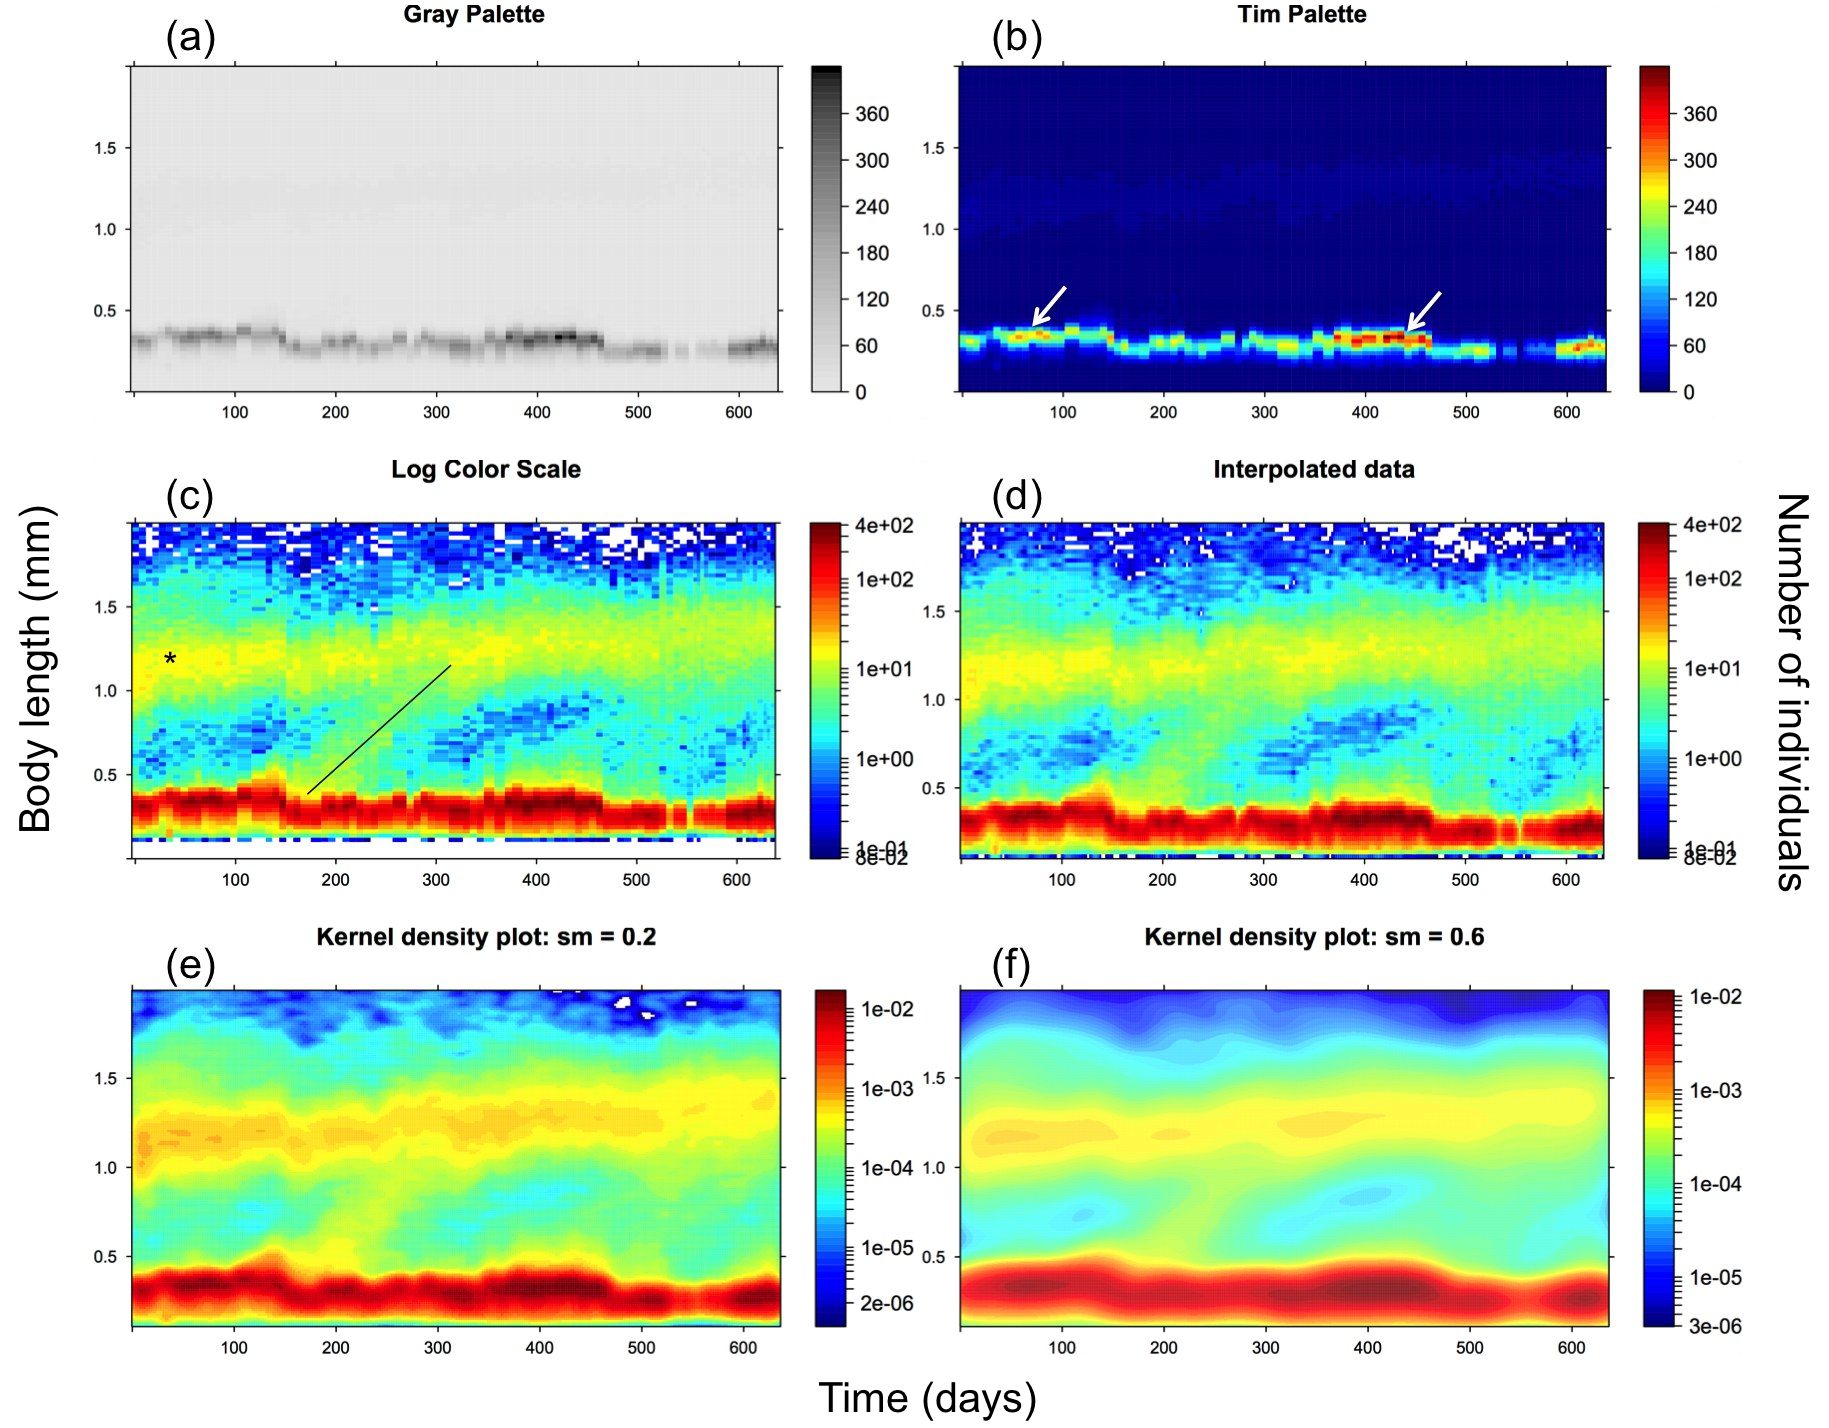
\includegraphics[width=0.95\textwidth]{1_CorpsDeThese/Methodo/STdiag2}
\caption[\lofimage{1_CorpsDeThese/Methodo/STdiag2} Diagrammes
structure-temps pour une population exemple]{Exemple de diagrammes
structure-temps de la population de collemboles de la Figure \ref{fig:STd1} pour
illustrer les possibilités offertes par la librairie \texttt{STdiag}. (a)
Palette de couleur sur une échelle de gris linéaire. (b) Palette de couleur
\texttt{tim.colors} linéaire. Les flèches blanches révèlent des pulses
d'éclosions de collemboles. (c) Palette de couleur logarithmique. L'étoile marque la taille adulte mesurée avec la fonction \texttt{STdiag.measure}. La ligne marque une cohorte mesurée avec la
fonction \texttt{STdiag.measure} dont le taux de croissance est la pente de la
droite. (e) Interpolation des données présentées en (c). (e) et (f) Deux
représentation lissées avec des largeurs de kernel différentes (option
\texttt{smooth=TRUE} et \texttt{sm}). }
\label{fig:STd2}
\end{center}
\end{figure}

\subsubsection{Mesure quantitatives sur le diagramme}

La librairie fournit une fonction \texttt{STdiag.measure} qui permet d'interagir
avec le diagramme pour sélectionner un point ou une ligne en cliquant dessus (un
clic pour le point, deux pour les extrémités de la ligne, voir Figure \ref{fig:STd2}c). Cette fonction fournit alors les coordonnées en $x$,
$y$ et $z$ du point cliqué ou des extrémités de la ligne sélectionnée. Dans le cas d'une ligne, la fonction
renvoie également la pente de la ligne sélectionnée dans le repère formé par
$(x,y)$. Enfin, les options \texttt{region} et \texttt{range} permettent
d'extraire des données initiales les points correspondant à une région autour du
point ou de la ligne sélectionnées.

\subsection{Lire et interpréter les diagrammes}

La Figure \ref{fig:STd2} illustre donc la dynamique d'une population de
collemboles élevées dans les conditions décrites précédemment. On constate
rapidement que la dynamique est dominée par des individus de petite taille
($\approx 0.5mm$, flèches blanches en b). De plus, la structure de la population
semble avoir une distribution bimodale stable, avec un groupe d'adultes autour
de $1.2mm$ (étoile en c). Ces diagrammes révèlent également des dynamiques
interclasses que l'on ne pouvait distinguer sur aucune des représentation de la
Figure \ref{fig:STd1}. Notamment, la ligne du panel (c) montre une cohorte qui
recrute depuis les juvéniles vers les adultes avec un taux de croissance
d'environ $0.22 mm/mois$. Enfin, il est possible d'observer des dynamiques au
long terme. En effet, la couleur jaune semble s'estomper dans le groupe d'adulte
alors que la taille moyenne augmente au cours des $600$ jours. Ainsi, il
semblerait que les adultes atteignent des tailles de plus en plus grandes alors
que leur nombre diminue légèrement. 

Ces diagrammes permettent ainsi d'entrer dans le détail de la dynamique de la
structure des populations. L'analyse détaillée de 28 populations de collembole des clones HA
et TO (16 HA et 12 TO) est présentée dans le Chapitre \ref{chap:sp} page
\pageref{chap:sp} ainsi que dans l'Annèxe \ref{Ann:SP}.



